\Opensolutionfile{ans}[ans/G12D2TN]
% ===================================================================
\begin{ex}
	Phát biểu nào sau đây về hằng số Avogadro là \textbf{sai}?	
	\choice
	{Hằng số Avogadro là số lượng nguyên tử trong $\SI{0.012}{\kilogram}$ carbon-12}
	{Giá trị của hằng số Avogadro là $\SI{6.02E23}{}$.}
	{Hằng số Avogadro là số phân tử có trong một mol chất}
	{\True Hằng số Avogadro chỉ áp dụng được cho các hạt đơn nguyên tử}
	\loigiai{}
\end{ex}
% ===================================================================
\begin{ex}
	Khối khí lí tưởng \textbf{không có} đặc điểm nào sau đây?
	\choice
	{Lực tương tác giữa các phân tử rất nhỏ trừ khi va chạm}
	{Thể tích các phân tử khí rất nhỏ so với thể tích của bình chứa}
	{\True Khi các phân tử khí va chạm nhau thì quá trình và chạm đó là va chạm không đàn hồi}
	{Gồm một số rất lớn các phân tử khí}
	\loigiai{}
\end{ex}
% ===================================================================
\begin{ex}
	Quá trình nào sau đây \textbf{không phải} là quá trình đẳng tích?
	\choice
	{\True Bọt khí nổi lên từ đáy một hồ nước}
	{Bánh xe đạp bị mềm hơn do nhiệt độ giảm}
	{Quả bóng cao su được phơi ngoài nắng}
	{Khối khí bị nhốt trong cylanh nhờ piston cố định}
	\loigiai{}
\end{ex}
% ===================================================================
\begin{ex}
	Hệ thức nào sau đây \textbf{phù hợp} với định luật Boyle?
	\choice
	{$\dfrac{p_1}{p_2}=\dfrac{V_1}{V_2}$}
	{\True $p_1V_1=p_2V_2$}
	{$\dfrac{p_1}{V_1}=\dfrac{p_2}{V_2}$}
	{$p\sim V$}
	\loigiai{}
\end{ex}
% ===================================================================
\begin{ex}
\immini{
Dựa vào đồ thị hình bên, hệ thức nào sau đây là \textbf{đúng}?	
\choice
{$p_1>p_2$}
{$p_1=p_2$}
{\True $p_1<p_2$}
{$p_1-p_2=2p_2$}
}{
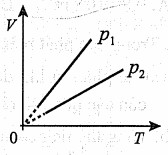
\includegraphics[width=0.4\linewidth]{../figs/G12-D2-1}
}
	\loigiai{}
\end{ex}
% ===================================================================
\begin{ex}
	Chọn câu \textbf{đúng}.\\
	Khi dãn nở đẳng nhiệt thì	
	\choice
	{\True số phân tử khí trong một đơn vị thể tích giảm}
	{khối lượng riêng của khí tăng lên}
	{áp suất khí tăng lên}
	{số phân tử khí trong một đơn vị thể tích tăng}
	\loigiai{}
\end{ex}
% ===================================================================
\begin{ex}
	Một bình chứa khí có thể tích không đổi, nếu áp suất giảm một nửa thì nhiệt độ tuyệt đối thay đổi như thế nào?	
	\choice
	{Tăng 2 lần}
	{\True Giảm 1 nửa}
	{Giảm 4 lần}
	{Tăng 4 lần}
	\loigiai{Trong quá trình biến đổi đẳng tích của một lượng khí xác định thì áp suất tỉ lệ thuận với nhiệt độ tuyệt đối.}
\end{ex}

% ===================================================================
\begin{ex}
	Đồ thị nào sau đây phù hợp với định luật Boyle đối với một lượng khí xác định ở hai nhiệt độ khác nhau $\left(T_1>T_2\right)$?	
	\begin{center}
		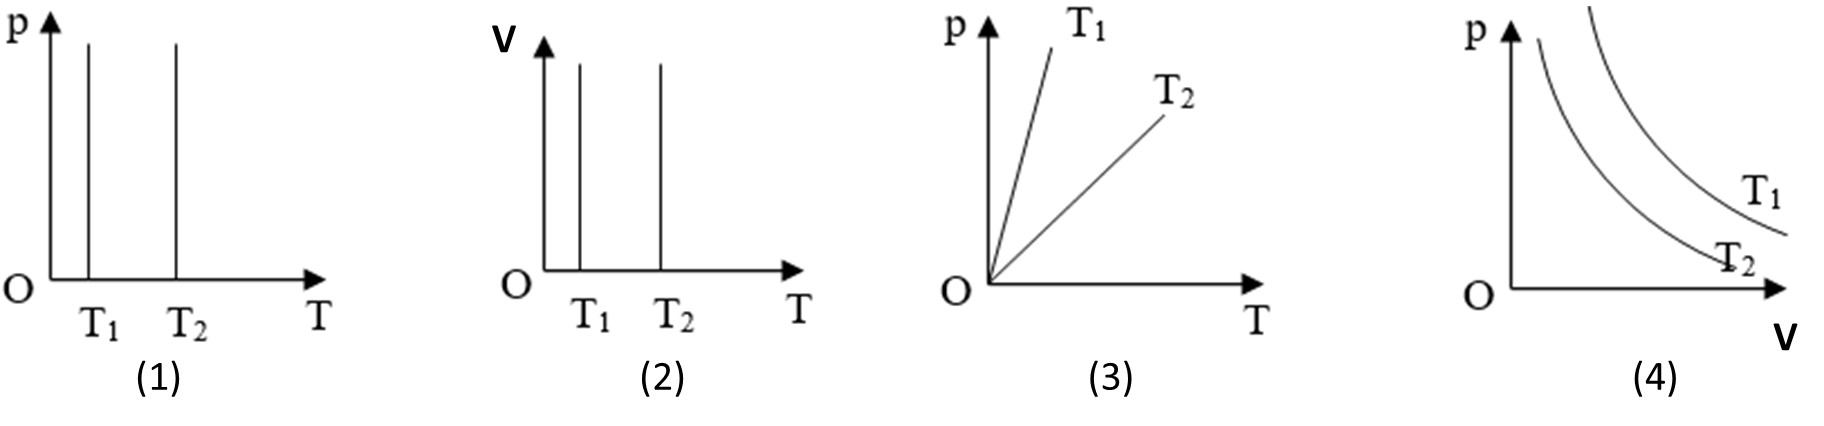
\includegraphics[width=0.65\linewidth]{../figs/G12-D2-2}
	\end{center}
	\choice
	{(1)}
	{(2)}
	{(3)}
	{\True (4)}
	\loigiai{}
\end{ex}
% ===================================================================
\begin{ex}
	Biểu thức nào dưới đây diễn tả đúng phương trình trạng thái khí lí tưởng?
	\choice
	{\True $\dfrac{pV}{T}=\text{const}$}
	{$p_1V_1T_1=p_2V_2T_2$}
	{$\dfrac{T_1V_1}{p_1}=\dfrac{T_2V_2}{p_2}$}
	{$\dfrac{T_1p_1}{V_1}=\dfrac{T_2p_2}{V_2}$}
	\loigiai{}
\end{ex}
% ===================================================================
\begin{ex}
	Nội năng của một khối khí lí tưởng không thay đổi trong quá trình nào sau đây?
	\choice
	{Đẳng tích}
	{Đẳng áp}
	{\True Đẳng nhiệt}
	{Bất kì}
	\loigiai{}
\end{ex}
% ===================================================================
\begin{ex}
	Quá trình biến đổi trạng thái của một lượng khí lí tưởng xác định mà áp suất tỉ lệ với số phân tử chứa trong một đơn vị thể tích là quá trình
	\choice
	{\True đẳng nhiệt}
	{đẳng tích}
	{đẳng áp}
	{không phải các quá trình đã nêu}
	\loigiai{
$pV=\dfrac{N}{N_\text{A}}RT\Rightarrow p=\nu \dfrac{R}{N_\text{A}}T$. Do đó, $p\sim \nu$ khi $T=\text{const}$.
}
\end{ex}

% ===================================================================
\begin{ex}
	Trong hệ toạ độ $\left(p, T\right)$, đường nào sau đây biểu diễn đường đẳng tích?
	\choice
	{Đường thẳng cắt trục $Op$ tại điểm $p=p_0$}
	{Đường cong hyperbol}
	{Đường thẳng vuông góc với trục $OT$}
	{\True Đường thẳng kéo dài đi qua gốc toạ độ}
	\loigiai{}
\end{ex}
% ===================================================================
\begin{ex}
	Khối khí trong một cylanh nhận nhiệt hay toả nhiệt một lượng bao nhiêu nếu như người ta thực hiện công $\SI{40}{\joule}$ lên khối khí và nội năng khối khí tăng thêm $\SI{20}{\joule}$?
	\choice
	{\True Khối khí toả nhiệt $\SI{20}{\joule}$}
	{Khối khí nhận nhiệt $\SI{20}{\joule}$}
	{Khối khí toả nhiệt $\SI{40}{\joule}$}
	{Khối khí nhận nhiệt $\SI{40}{\joule}$}
	\loigiai{
$\Delta U=Q+A\Rightarrow Q=\Delta U-A=-\SI{20}{\joule}$. Vì $Q<0$ nên khối khí đã toả nhiệt $\SI{20}{\joule}$.	
}
\end{ex}
% ===================================================================
\begin{ex}
Cho 1 cylanh chứa $\SI{300}{\centi\meter^3}$ khí ở áp suất $\SI{2E5}{\pascal}$. Piston nén khí trong cylanh xuống còn $\SI{100}{\centi\meter^3}$. Coi nhiệt độ không đổi. Áp suất của khí trong cylanh nhận giá trị nào sau đây?	
	\choice
	{$\SI{3.5E5}{\pascal}$}
	{$\SI{3E5}{\pascal}$}
	{$\SI{E5}{\pascal}$}
	{\True $\SI{6E5}{\pascal}$}
	\loigiai{
	$p_1V_1=p_2V_2\Rightarrow p_2=\dfrac{p_1V_1}{V_2}=\SI{6E5}{\pascal}$.}
\end{ex}
% ===================================================================
\begin{ex}
	Một khối khí lí tưởng có thể tích $\SI{10}{\liter}$ đang ở áp suất $\SI{1.6}{atm}$ thì được nén đẳng nhiệt cho đến khi áp suất bằng $\SI{4}{atm}$. Thể tích của khối khí đã thay đổi
	\choice
	{$\SI{2.5}{\liter}$}
	{$\SI{6.25}{\liter}$}
	{\True $\SI{4}{\liter}$}
	{$\SI{6}{\liter}$}
	\loigiai{
$p_1V_1=p_2V_2\Rightarrow V_2=\dfrac{p_1V_1}{p_2}=\SI{4}{\liter}.$	
}
\end{ex}
% ===================================================================
\begin{ex}
Một bình đựng khí oxygen có thể tích $\SI{150}{\milli\liter}$ và áp suất bằng $\SI{450}{\kilo\pascal}$. Coi nhiệt độ không đổi. Thể tích của khí này là bao nhiêu khi áp suất của khí là $\SI{150}{\kilo\pascal}$?
	\choice
	{$\SI{50}{\milli\liter}$}
	{\True $\SI{450}{\milli\liter}$}
	{$\SI{100}{\milli\liter}$}
	{$\SI{300}{\milli\liter}$}
	\loigiai{
Áp dụng định luật Boyle:
$$p_1V_1=p_2V_2\Rightarrow V_2=\SI{450}{\milli\liter}.$$	
}
\end{ex}
% ===================================================================
\begin{ex}
Một cylanh chứa khí ở áp suất $\SI{3E5}{\pascal}$, nhiệt độ $\SI{300}{\kelvin}$. Để giảm áp suất khí xuống còn $\SI{1.5E5}{\pascal}$ trong điều kiện thể tích không đổi thì cần điều chỉnh nhiệt độ khí trong xilanh đến
	\choice
	{\True $\SI{150}{\kelvin}$}
	{$\SI{400}{\kelvin}$}
	{$\SI{200}{\kelvin}$}
	{$\SI{100}{\kelvin}$}
	\loigiai{
Trong điều kiện đẳng tích:
$$\dfrac{T_2}{T_1}=\dfrac{p_2}{p_1}=\dfrac{1}{2}\Rightarrow T_2=\dfrac{T_1}{2}=\SI{150}{\kelvin}.$$	
}
\end{ex}
% ===================================================================
\begin{ex}
	Có $\SI{2.00}{\mole}$ khí nitrogen đựng trong một xilanh kín. Biết số khối của nitrogen là 28. Có bao nhiêu gram nitrogen trong xilanh?
	\choice
	{$\SI{0.14}{}$}
	{\True $\SI{56}{}$}
	{$\SI{42}{}$}
	{$\SI{112}{}$}
	\loigiai{$m=nA=\SI{56}{\gram}.$}
\end{ex}
% ===================================================================
\begin{ex}
	Một khối khí lí tưởng đang ở nhiệt độ $\SI{87}{\celsius}$ thì được làm lạnh cho tới khi áp suất giảm còn một nửa, nhiệt độ giảm đi $2/3$ lần. Sau khi làm lạnh, thể tích khối khí là $\SI{6}{\liter}$. Thể tích khối khí trước khi làm lạnh là
	\choice
	{ $\SI{3.26}{\liter}$}
	{\True$\SI{3.58}{\liter}$}
	{$\SI{2}{\liter}$}
	{$\SI{2.76}{\liter}$}
	\loigiai{
		\colorbox{cyan!35}{Đề bài cho nhiệt độ giảm 2/3 chứ không phải nhiệt độ tuyệt đối giảm nên $t_2=\dfrac{t_1}{3}$.}
\begin{center}
	\begin{tabular}{C{6cm} C{3cm} C{6cm}}
		\colorbox{yellow}{\textcolor{red}{\textbf{Trạng thái 1}}} & $\xrightarrow[]{n=\text{const}}$ & \colorbox{yellow}{\textcolor{red}{\textbf{Trạng thái 2}}}\\
		$t_1=\SI{87}{\celsius}\Rightarrow T_1=\SI{360}{\kelvin}$ & &$t_2=\dfrac{1}{3}t_1=\SI{29}{\celsius}\Rightarrow T_2=\SI{302}{\kelvin}$\\
		$p_1$ & & $p_2=0,5p_1$\\
		$V_1=?$& & $V_2=\SI{6}{\liter}$
	\end{tabular}
	
\end{center}	
Áp dụng phương trình trạng thái khí lí tưởng:
$$\dfrac{p_1V_1}{T_1}=\dfrac{p_2V_2}{T_2}\Rightarrow V_1\approx \SI{3.58}{\liter}.$$

}
\end{ex}
% ===================================================================
\begin{ex}
	\immini{
Một khối khí lí tưởng thực hiện quá trình biến đổi trạng thái như đồ thị hình bên. Khối khí đã thực hiện công hay nhận công bao nhiêu?	

}{	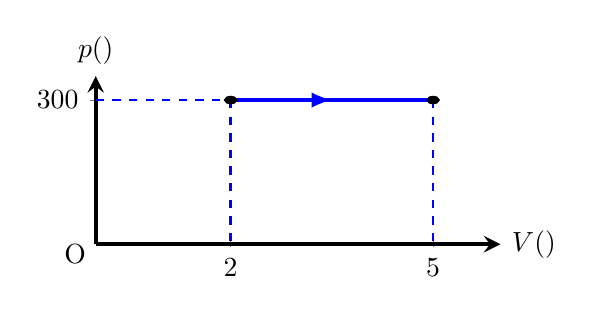
\begin{tikzpicture}  
		\begin{axis}[  ultra thick, scale=0.75,  yscale=0.5,
			xmin=0,  
			xmax=6,  
			ytick={300},
			xtick={2,5},
			ymin=0,  
			ymax=350, 
			samples=300,
			axis lines=center, 
			xlabel=$\xsi{V}{\left(\liter\right)}$, 
			ylabel=$\xsi{p}{\left(\kilo\pascal\right)}$, 
			every axis y label/.style={at=(current axis.above origin),anchor=south},  
			every axis x label/.style={at=(current axis.right of origin),anchor=west},  ]
			\draw[line width=1pt,blue, dashed] (axis cs: 0, 300) -- (axis cs: 5, 300);
			\draw[line width=1pt,blue, dashed] (axis cs: 2, 300) -- (axis cs: 2, 0);
			\draw[line width=1pt,blue, dashed] (axis cs: 5, 300) -- (axis cs:5, 0);
			\draw[line width=1.5pt,blue] (axis cs: 2, 300) -- (axis cs: 5, 300);
			\draw[line width=1.5pt,blue,-latex] (axis cs: 2, 300) -- (axis cs: 3.5, 300);
			\filldraw[black] (axis cs:2,300) circle (1.5pt);
			\filldraw[black] (axis cs:5,300) circle (1.5pt);
		\end{axis}  
		\node[label={[below left]90:O}] at (0,0){};
	\end{tikzpicture}
}
\choice
{$\SI{0.6}{\kilo\joule}$}
{\True $\SI{0.9}{\kilo\joule}$}
{$\SI{1.5}{\kilo\joule}$}
{$\SI{1.2}{\kilo\joule}$}	
	\loigiai{$A=p\Delta V=\SI{0.9}{\kilo\joule}$.
	}
\end{ex}
% ===================================================================
\begin{ex}
Có một lượng khí lí tưởng đựng trong bình, áp suất của khí sẽ biến đổi như thế nào nếu thể tích của bình tăng gấp 3 lần, nhiệt độ tuyệt đối giảm 1 nửa?	
	\choice
	{Tăng 1,5 lần}
	{Giảm 1,5 lần}
	{\True Giảm đi 6 lần}
	{Tăng gấp 6 lần}
	\loigiai{
$p=\dfrac{nRT}{V}\Rightarrow \dfrac{p'}{p}=\dfrac{T'}{T}\cdot \dfrac{V}{V'}=\dfrac{1}{6}.$	
}
\end{ex}
% ===================================================================
\begin{ex}
	Ở nhiệt độ $T_1$, áp suất khí là $p_1$, khối lượng riêng $\rho_1$. Biểu thức khối lượng riêng của khí trên ở nhiệt độ $T_2$ và áp suất $p_2$ là
	\choice
	{$\rho_2=\dfrac{p_2T_2}{p_1T_1}\rho_1$}
	{$\rho_2=\dfrac{p_1T_1}{p_2T_2}\rho_1$}
	{\True $\rho_2=\dfrac{p_2T_1}{p_1T_2}\rho_1$}
	{$\rho_2=\dfrac{p_1T_2}{p_2T_1}\rho_1$}
	\loigiai{
	Từ $pV=\dfrac{m}{M}RT\Rightarrow \rho=\dfrac{pM}{RT}\Rightarrow \dfrac{\rho_2}{\rho_1}=\dfrac{p_2T_1}{p_1T_2}.$
}
\end{ex}

% ===================================================================
\begin{ex}
	Khối lượng riêng của một lượng khí ở áp suất $\SI{2E5}{\pascal}$ là $\SI{1.5}{\kilogram/\meter^3}$. Nhiệt độ khí không đổi, khối lượng riêng của khí đó ở $\SI{6E5}{\pascal}$ nhận giá trị nào sau đây?
	\choice
	{$\SI{0.5}{\kilogram/\meter^3}$}
	{\True $\SI{4.5}{\kilogram/\meter^3}$}
	{$\SI{2}{\kilogram/\meter^3}$}
	{$\SI{3}{\kilogram/\meter^3}$}
	\loigiai{
Từ $pV=\dfrac{m}{M}RT\Rightarrow \rho=\dfrac{pM}{RT}.$\\
Vì nhiệt độ khối khí không đổi nên:
$$\dfrac{\rho'}{\rho}=\dfrac{p'}{p}\Rightarrow \rho'=\SI{4.5}{\kilogram/\meter^3}.$$	
}
\end{ex}
% ===================================================================
\begin{ex}
Một bình có dung tích $\SI{9.52}{\liter}$ chứa $\SI{0.85}{\mole}$ khí ở $\SI{0}{\celsius}$. Áp suất khí trong bình là	
	\choice
	{$\SI{2.85}{atm}$}
	{$\SI{1.7}{atm}$}
	{\True $\SI{2}{atm}$}
	{một giá trị khác}
	\loigiai{
Áp dụng phương trình Clapeyron - Mendeleev:
$$pV=nRT\Rightarrow p=\dfrac{nRT}{V}=\SI{202556.25}{\pascal}\approx\SI{2}{atm}.$$	
}
\end{ex}
% ===================================================================
\begin{ex}
	\immini{
	Một khối khí lí tưởng thực hiện quá trình biến đổi trạng thái (1)-(2)-(3) như đồ thị hình bên. Các thông số được cho trên đồ thị. Biết áp suất của chất khí khi bắt đầu quá trình là $\SI{12}{atm}$. Áp suất của khối khí khi kết thúc quá trình là
}{
	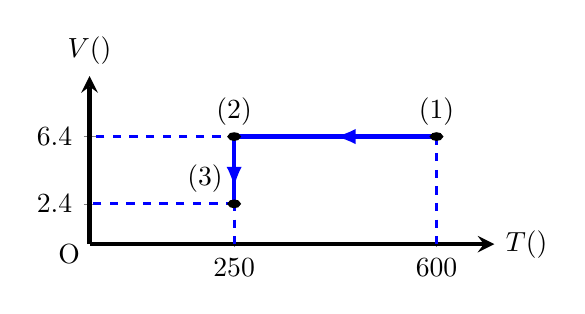
\begin{tikzpicture}  
		\begin{axis}[  ultra thick, scale=0.75, yscale=0.5,
			xmin=0,  
			xmax=700,  
			ytick={2.4, 6.4},
			xtick={250,600},
			ymin=0,  
			ymax=10, 
			samples=300,
			axis lines=center, 
			xlabel=$\xsi{T}{\left(\kelvin\right)}$, 
			ylabel=$\xsi{V}{\left(\liter\right)}$, 
			every axis y label/.style={at=(current axis.above origin),anchor=south},  
			every axis x label/.style={at=(current axis.right of origin),anchor=west},  ]
			\draw[line width=1pt,blue, dashed] (axis cs: 600, 6.4) -- (axis cs: 0, 6.4);
			\draw[line width=1pt,blue, dashed] (axis cs: 250, 6.4) -- (axis cs: 250, 0);
			\draw[line width=1pt,blue, dashed] (axis cs: 250, 2.4) -- (axis cs:0, 2.4);
			\draw[line width=1pt,blue, dashed] (axis cs: 600, 6.4) -- (axis cs: 600, 0);
			\draw[line width=1.5pt,blue] (axis cs: 600, 6.4) -- (axis cs: 250, 6.4);
			\draw[line width=1.5pt,blue] (axis cs: 250, 6.4) -- (axis cs: 250, 2.4);
			\draw[line width=1.5pt,blue,-latex] (axis cs: 600, 6.4) -- (axis cs: 425, 6.4);
			\draw[line width=1.5pt,blue, -latex] (axis cs: 250, 6.4) -- (axis cs: 250, 3.4);
			\filldraw[black] (axis cs:600,6.4) circle (1.5pt) node[above] {(1)};
			\filldraw[black] (axis cs:250,6.4) circle (1.5pt) node[above] {(2)};
			\filldraw[black] (axis cs:250,2.4) circle (1.5pt) node[above left] {(3)};
		\end{axis}  
		\node[label={[below left]90:O}] at (0,0){};
	\end{tikzpicture}
}
	\choice
	{$\SI{1.875}{atm}$}
	{$\SI{5}{atm}$}
	{\True $\SI{13.33}{atm}$}
	{$\SI{2.67}{atm}$}
	\loigiai{
Áp dụng phương trình trạng thái khí lí tưởng:
$$\dfrac{p_1V_1}{T_1}=\dfrac{p_2V_2}{T_2}\Rightarrow p_2=\SI{13.33}{atm}.$$	
}
\end{ex}
% ===================================================================
\begin{ex}
	Có $\SI{14}{\gram}$ chất khí nào đó đựng trong bình kín có thể tích $\SI{1}{\liter}$. Đun nóng đến $\SI{127}{\celsius}$ áp suất khí trong bình là $\SI{16.62E5}{\pascal}$. Khí đó là khí
	\choice
	{helium}
	{\True nitrogen}
	{hydrogen}
	{oxygen}
	\loigiai{
$$pV=\dfrac{m}{M}RT\Rightarrow M=\dfrac{mRT}{pV}=\SI{28}{\gram/\mole}.$$
}
\end{ex}


% ===================================================================
\begin{ex}
	Một khối khí lí tưởng có thể tích $\SI{10}{\liter}$, nhiệt độ $\SI{27}{\celsius}$, áp suất $\SI{1}{atm}$ biến đổi qua 2 quá trình
	\begin{enumerate}[label= Quá trình \arabic*:, leftmargin=2.5cm]
		\item đẳng tích, áp suất tăng gấp 2 lần.
		\item đẳng áp, thể tích sau cùng là $\SI{15}{\liter}$.
	\end{enumerate}
	Nhiệt độ sau cùng của khí là
	\choice
	{$\SI{90}{\kelvin}$}
	{\True $\SI{900}{\kelvin}$}
	{$\SI{9000}{\kelvin}$}
	{một giá trị khác}
	\loigiai{
		\begin{center}
			\begin{tabular}{C{3cm} C{2cm} C{3cm} C{2cm} C{3cm}}
				\colorbox{yellow}{\textcolor{red}{\textbf{Trạng thái 1}}} & $\xrightarrow{V=\text{const}}$ & \colorbox{yellow}{\textcolor{red}{\textbf{Trạng thái 2}}}& $\xrightarrow{p=\text{const}}$ & \colorbox{yellow}{\textcolor{red}{\textbf{Trạng thái 3}}}\\
				$p_1=\SI{1}{atm}$ & &$p_2=2p_1=\SI{2}{atm}$ && $p_3=p_2=\SI{2}{atm}$\\
				$V_1=\SI{10}{\liter}$ & & $V_2=\SI{10}{\liter}$ & & $V_3=\SI{15}{\liter}$\\
				$T_1=\SI{300}{\kelvin}$ & &  & & $T_3=?$
			\end{tabular}
		\end{center}
		Áp dụng phương trình trạng thái khí lí tưởng:
		$$\dfrac{p_1V_1}{T_1}=\dfrac{p_3V_3}{T_3}\Rightarrow T_3=\dfrac{p_3V_3}{p_1V_1}T_1=\SI{900}{\kelvin}.$$
	}
\end{ex}
% ===================================================================
\begin{ex}
Một bình chứa khí ở nhiệt độ $\SI{53}{\celsius}$ và áp suất $\SI{28}{atm}$. Người ta cho $1/3$ lượng khí thoát ra khỏi bình và hạ nhiệt độ còn $\SI{17}{\celsius}$. Áp suất khí còn lại trong bình là	
	\choice
	{$\SI{8.3}{atm}$}
	{$\SI{166}{atm}$}
	{$\SI{5.98}{atm}$}
	{\True $\SI{16.6}{atm}$}
	\loigiai{
Ta có:
\begin{equation}
	p_1V=nRT_1
	\label{eq: 1}
\end{equation}	\\
\begin{equation}
	p_2V=\dfrac{2n}{3}RT_2
	\label{eq: 2}
\end{equation}	
Từ \eqref{eq: 1} và \eqref{eq: 2}, thu được:
$$\dfrac{p_2}{p_1}=\dfrac{2T_2}{3T_1}\Rightarrow p_2=\dfrac{T_2}{3T_1}p_1\approx\SI{16.6}{atm}.$$
}
\end{ex}

% ===================================================================
\begin{ex}
Ở nhiệt độ nào thì căn bậc hai của trung bình bình phương tốc độ các phân tử khí oxygen $\left(\ce{O_2}\right)$ đạt tốc độ vũ trụ cấp I $\left(\SI{7.9}{\kilo\meter/\second}\right)$?	
	\choice
	{$\SI{6.0E4}{\kelvin}$}
	{$\SI{4.0E4}{\kelvin}$}
	{\True $\SI{8.0E4}{\kelvin}$}
	{$\SI{2.0E4}{\kelvin}$}
	\loigiai{$\overline{v^2}=\dfrac{3RT}{M}\Rightarrow T=\dfrac{M\overline{v^2}}{3R}=\dfrac{\left(\SI{7.9E3}{\meter/\second}\right)^2\cdot\left(\SI{32E-3}{\kilogram/\mole}\right)}{3\cdot\left(\SI{8.31}{\joule\mole^{-1}\kelvin^{-1}}\right)}\approx\SI{8.0E4}{\kelvin}.$}
\end{ex}
% ===================================================================
\begin{ex}
$\SI{1.4}{\mole}$ khí lí tưởng thực hiện quá trình biến đổi trạng thái như đồ thị hình bên. Biết nhiệt lượng mà khối khí nhận được trong quá trình trên là $\SI{1154}{\joule}$. Độ biến thiên nội năng của khối khí bằng
\begin{center}
	\begin{tikzpicture}  
		\begin{axis}[  ultra thick,
			xmin=0,  
			xmax=400,  
			ytick={1, 1.7},
			xtick={200, 340},
			yticklabels={$V_1$, $V_2$},
			xticklabels={300, 340},
			ymin=0,  
			ymax=2, 
			samples=300,
			axis lines=center, 
			xlabel=$\xsi{T}{\left(\kelvin\right)}$, 
			ylabel=$V$, 
			every axis y label/.style={at=(current axis.above origin),anchor=south},  
			every axis x label/.style={at=(current axis.right of origin),anchor=west},  ]
			\coordinate (O) at  (axis cs: 0, 0);
			\coordinate (A) at  (axis cs: 200, 1);
			\coordinate (B) at  (axis cs: 340, 1.7);
			\coordinate (M) at ($(A)!0.5!(B)$);
			\draw[line width=1pt,blue, dashed] (A) -- (axis cs: 200, 0);
			\draw[line width=1pt,blue, dashed] (A) -- (O);
			\draw[line width=1pt,blue, dashed] (A) -- (axis cs: 0, 1);
			\draw[line width=1pt,blue, dashed] (B) -- (axis cs: 340, 0);
			\draw[line width=1pt,blue, dashed] (B) -- (axis cs: 0, 1.7);
			\draw[line width=1.5pt,blue] (A) -- (B);
			\draw[line width=1.5pt,blue, -latex] (A) -- (M);
			\filldraw[black] (A) circle (1.5pt) node[above] {(1)};
			\filldraw[black] (B) circle (1.5pt) node[above right] {(2)};
		\end{axis}  
		\node[label={[below left]90:O}] at (0,0){};
	\end{tikzpicture}
\end{center}

	\choice
	{\True $\SI{689}{\kilo\joule}$}
	{$\SI{465}{\kilo\joule}$}
	{$\SI{1154}{\kilo\joule}$}
	{$\SI{1619}{\kilo\joule}$}
	\loigiai{
		Quá trình biến đổi (1) - (2) là quá trình đẳng áp vì $V$ tỉ lệ thuận với $T$.\\
Công mà khối khí thực hiện:
$$A'=p\left(V_2-V_1\right)=nR\left(T_2-T_1\right)=\SI{465.36}{\joule}.$$
Độ biến thiên nội năng của khối khí:
$$\Delta U=Q+A=Q-A'\approx\SI{689}{\joule}.$$	

}
\end{ex}

\Closesolutionfile{ans}
\begin{center}
	\textbf{--- HẾT ---}
\end{center}